%%%%%%%%%%%%%%%%%%%%%%%%%%%%%%%%%%%%%%%%%%%%%%%%%%%
\begin{frame}
  \begin{center}
    {\Large LSTM with Pytorch}
    
  \end{center}
\end{frame}


%%%%%%%%%%%%%%%%%%%%%%%%%%%%%%%%%%%%%%%%%%%%%%%%%%%
\begin{frame}[fragile] \frametitle{Long Short Term Memory (LSTM)}


\begin{itemize}
\item  One of the main problems of classical RNNs is so-called vanishing gradients problem. 
\item  Because RNNs are trained end-to-end in one back-propagation pass, it is having hard times propagating error to the first layers of the network, and thus the network cannot learn relationships between distant tokens. 
\item  One of the ways to avoid this problem is to introduce explicit state management by using so called gates. 
\item  There are two most known architectures of this kind: Long Short Term Memory (LSTM) and Gated Relay Unit (GRU).
\end{itemize}

\begin{center}
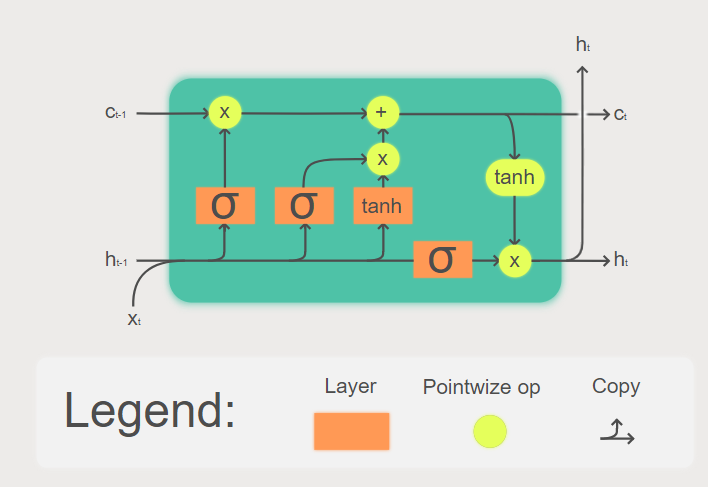
\includegraphics[width=0.4\linewidth,keepaspectratio]{pyt55}
\end{center}

\end{frame}

%%%%%%%%%%%%%%%%%%%%%%%%%%%%%%%%%%%%%%%%%%%%%%%%%%%
\begin{frame}[fragile] \frametitle{Long Short Term Memory (LSTM)}


\begin{itemize}
\item LSTM Network is organized in a manner similar to RNN, but there are two states that are being passed from layer to layer: actual state $c$, and hidden vector $h$. \item At each unit, hidden vector $h_i$ is concatenated with input $x_i$, and they control what happens to the state $c$ via gates. 
\item Each gate is a neural network with sigmoid activation (output in the range $[0,1]$), which can be thought of as bitwise mask when multiplied by the state vector. There are the following gates (from left to right on the picture above):

\begin{itemize}
\item forget gate: takes hidden vector and determines, which components of the vector $c$ we need to forget, and which to pass through. 
\item input gate: takes some information from the input and hidden vector, and inserts it into state.
\item output gate: transforms state via some linear layer with $\tanh$ activation, then selects some of its components using hidden vector $h_i$ to produce new state $c_{i+1}$.
\end{itemize}

\end{itemize}


\end{frame}

%%%%%%%%%%%%%%%%%%%%%%%%%%%%%%%%%%%%%%%%%%%%%%%%%%%
\begin{frame}[fragile] \frametitle{Long Short Term Memory (LSTM)}


\begin{itemize}

\item Components of the state $c$ can be thought of as some flags that can be switched on and off. 
\item For example, when we encounter a name $Alice$ in the sequence, we may want to assume that it refers to female character, and raise the flag in the state that we have female noun in the sentence. 
\item When we further encounter phrases $and$ $Tom$, we will raise the flag that we have plural noun. 
\item Thus by manipulating state we can supposedly keep track of grammatical properties of sentence parts.

\end{itemize}


\end{frame}

%%%%%%%%%%%%%%%%%%%%%%%%%%%%%%%%%%%%%%%%%%%%%%%%%%%
\begin{frame}[fragile] \frametitle{Long Short Term Memory (LSTM)}


\begin{itemize}
\item While internal structure of LSTM cell may look complex, PyTorch hides this implementation inside LSTMCell class, and provides LSTM object to represent the whole LSTM layer. 
\item Thus, implementation of LSTM classifier will be pretty similar to the simple RNN which we have seen above:

\end{itemize}

\begin{lstlisting}
class LSTMClassifier(torch.nn.Module):
    def __init__(self, vocab_size, embed_dim, hidden_dim, num_class):
        super().__init__()
        self.hidden_dim = hidden_dim
        self.embedding = torch.nn.Embedding(vocab_size, embed_dim)
        self.embedding.weight.data = torch.randn_like(self.embedding.weight.data)-0.5
        self.rnn = torch.nn.LSTM(embed_dim,hidden_dim,batch_first=True)
        self.fc = torch.nn.Linear(hidden_dim, num_class)

    def forward(self, x):
        batch_size = x.size(0)
        x = self.embedding(x)
        x,(h,c) = self.rnn(x)
        return self.fc(h[-1])
\end{lstlisting}

\end{frame}

%%%%%%%%%%%%%%%%%%%%%%%%%%%%%%%%%%%%%%%%%%%%%%%%%%%
\begin{frame}[fragile] \frametitle{Training LSTM}

Now let's train our network. 

\begin{itemize}
\item Note that training LSTM is also quite slow, and you may not seem much raise in accuracy in the beginning of training. 
\item Also, you may need to play with lr learning rate parameter to find the learning rate that results in reasonable training speed, and yet does not cause

\end{itemize}

\begin{lstlisting}
net = LSTMClassifier(vocab_size,64,32,len(classes)).to(device)
train_epoch(net,train_loader, lr=0.001)

>>>
3200: acc=0.259375
6400: acc=0.25859375
:
115200: acc=0.7677777777777778
118400: acc=0.7711233108108108
(0.03487814127604167, 0.7728)
\end{lstlisting}

\end{frame}


%%%%%%%%%%%%%%%%%%%%%%%%%%%%%%%%%%%%%%%%%%%%%%%%%%%
\begin{frame}[fragile] \frametitle{Packed sequences}

\begin{itemize}
\item  To produce packed sequence, we can use \lstinline|torch.nn.utils.rnn.pack_padded_sequence| function. 
\item All recurrent layers, including RNN, LSTM and GRU, support packed sequences as input, and produce packed output, which can be decoded using \lstinline|torch.nn.utils.rnn.pad_packed_sequence|.
\item To be able to produce packed sequence, we need to pass length vector to the network, and thus we need a different function to prepare minibatches:
\end{itemize}

\begin{lstlisting}
def pad_length(b):
    v = [encode(x[1]) for x in b] # build vectorized sequence
    # compute max length of a sequence in this minibatch and length sequence
    len_seq = list(map(len,v))
    l = max(len_seq)
    return ( # tuple - labels, padded features, length sequence
        torch.LongTensor([t[0]-1 for t in b]),
        torch.stack([torch.nn.functional.pad(torch.tensor(t),(0,l-len(t)),
				mode='constant',value=0) for t in v]),
        torch.tensor(len_seq)
    )

train_loader_len = torch.utils.data.DataLoader(train_dataset, batch_size=16, collate_fn=pad_length, shuffle=True)
\end{lstlisting}

\end{frame}

%%%%%%%%%%%%%%%%%%%%%%%%%%%%%%%%%%%%%%%%%%%%%%%%%%%
\begin{frame}[fragile] \frametitle{Packed sequences}

\begin{itemize}
\item  Actual network would be very similar to LSTMClassifier above, but forward pass will receive both padded minibatch and the vector of sequence lengths. 
\item After computing the embedding, we compute packed sequence, pass it to LSTM layer, and then unpack the result back.
\end{itemize}

Note:
\begin{itemize}
\item   We actually do not use unpacked result $x$, because we use output from the hidden layers in the following computations. 
\item Thus, we can remove the unpacking altogether from this code. 
\item The reason we place it here is for you to be able to modify this code easily, in case you should need to use network output in further computations.
\end{itemize}

\end{frame}

%%%%%%%%%%%%%%%%%%%%%%%%%%%%%%%%%%%%%%%%%%%%%%%%%%%
\begin{frame}[fragile] \frametitle{Packed sequences}



\begin{lstlisting}
class LSTMPackClassifier(torch.nn.Module):
    def __init__(self, vocab_size, embed_dim, hidden_dim, num_class):
        super().__init__()
        self.hidden_dim = hidden_dim
        self.embedding = torch.nn.Embedding(vocab_size, embed_dim)
        self.embedding.weight.data = torch.randn_like(self.embedding.weight.data)-0.5
        self.rnn = torch.nn.LSTM(embed_dim,hidden_dim,batch_first=True)
        self.fc = torch.nn.Linear(hidden_dim, num_class)

    def forward(self, x, lengths):
        batch_size = x.size(0)
        x = self.embedding(x)
        pad_x = torch.nn.utils.rnn.pack_padded_sequence(x,lengths,batch_first=True,enforce_sorted=False)
        pad_x,(h,c) = self.rnn(pad_x)
        x, _ = torch.nn.utils.rnn.pad_packed_sequence(pad_x,batch_first=True)
        return self.fc(h[-1])
\end{lstlisting}

\end{frame}

%%%%%%%%%%%%%%%%%%%%%%%%%%%%%%%%%%%%%%%%%%%%%%%%%%%
\begin{frame}[fragile] \frametitle{LSTM Classifier Training}

Note: You may have noticed the \lstinline|parameter use_pack_sequence| that we pass to the training function. Currently, \lstinline|pack_padded_sequence| function requires length sequence tensor to be on CPU device, and thus training function needs to avoid moving the length sequence data to GPU when training

\begin{lstlisting}
net = LSTMPackClassifier(vocab_size,64,32,len(classes)).to(device)
train_epoch_emb(net,train_loader_len, lr=0.001,use_pack_sequence=True)

>>>
3200: acc=0.285625
6400: acc=0.33359375
:
115200: acc=0.8104600694444445
118400: acc=0.8128293918918919
(0.029785829671223958, 0.8138166666666666)
\end{lstlisting}



\end{frame}

%%%%%%%%%%%%%%%%%%%%%%%%%%%%%%%%%%%%%%%%%%%%%%%%%%%
\begin{frame}[fragile] \frametitle{Bidirectional and multilayer RNNs}

\begin{itemize}
\item In many practical cases we have random access to the input sequence, it might make sense to run recurrent computation in both directions. Such networks are call bidirectional RNNs, and they can be created by passing \lstinline|bidirectional=True| parameter to RNN/LSTM/GRU constructor.
\item When dealing with bidirectional network, we would need two hidden state vectors, one for each direction. 
\item PyTorch encodes those vectors as one vector of twice larger size, which is quite convenient, because you would normally pass the resulting hidden state to fully-connected linear layer, and you would just need to take this increase in size into account when creating the layer.
\end{itemize}
\end{frame}

%%%%%%%%%%%%%%%%%%%%%%%%%%%%%%%%%%%%%%%%%%%%%%%%%%%
\begin{frame}[fragile] \frametitle{Bidirectional and multilayer RNNs}

\begin{itemize}
\item Recurrent network, one-directional or bidirectional, captures certain patterns within a sequence, and can store them into state vector or pass into output. 
\item As with convolutional networks, we can build another recurrent layer on top of the first one to capture higher level patterns, build from low-level patterns extracted by the first layer. 
\item This leads us to the notion of multi-layer RNN, which consists of two or more recurrent networks, where output of the previous layer is passed to the next layer as input.
\end{itemize}

\begin{center}
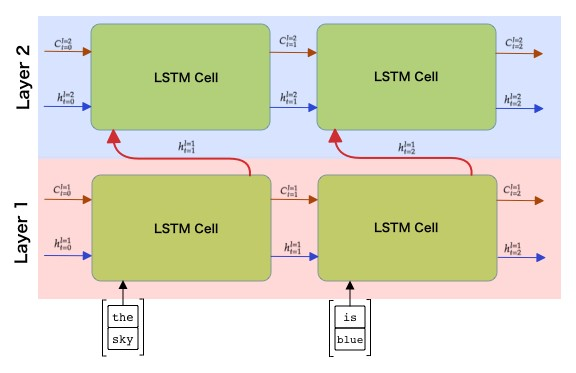
\includegraphics[width=0.6\linewidth,keepaspectratio]{pyt56}
\end{center}

{\tiny Picture from https://towardsdatascience.com/from-a-lstm-cell-to-a-multilayer-lstm-network-with-pytorch-2899eb5696f3}

\end{frame}

%%%%%%%%%%%%%%%%%%%%%%%%%%%%%%%%%%%%%%%%%%%%%%%%%%%
\begin{frame}[fragile] \frametitle{Summary}

\begin{itemize}
\item PyTorch makes constructing such networks an easy task, because you just need to pass \lstinline|num_layers| parameter to RNN/LSTM/GRU constructor to build several layers of recurrence automatically. 
\item This would also mean that the size of hidden/state vector would increase proportionally, and you would need to take this into account when handling the output of recurrent layers.
\end{itemize}


\end{frame}


%%%%%%%%%%%%%%%%%%%%%%%%%%%%%%%%%%%%%%%%%%%%%%%%%%%
\begin{frame}[fragile] \frametitle{Packed sequences}

\begin{itemize}
\item In our example, we had to pad all sequences in the minibatch with zero vectors. 
\item While it results in some memory waste, with RNNs it is more critical that additional RNN cells are created for the padded input items, which take part in training, yet do not carry any important input information. 
\item It would be much better to train RNN only to the actual sequence size.
\item To do that, a special format of padded sequence storage is introduced in PyTorch. 
\end{itemize}



\end{frame}


%%%%%%%%%%%%%%%%%%%%%%%%%%%%%%%%%%%%%%%%%%%%%%%%%%%
\begin{frame}[fragile] \frametitle{Packed sequences}

\begin{itemize}
\item Suppose we have input padded minibatch which looks like this:

\item Here 0 represents padded values, and the actual length vector of input sequences is $[5,3,1]$ (Read length vertically!!).

\item In order to effectively train RNN with padded sequence, we want to begin training first group of RNN cells with large minibatch ($[1,6,9]$), but then end processing of third sequence, and continue training with shorted minibatches ($[2,7]$, $[3,8]$), and so on. 
\item Thus, packed sequence is represented as one vector - in our case $[1,6,9,2,7,3,8,4,5]$, and length vector ($[5,3,1]$), from which we can easily reconstruct the original padded minibatch.
\end{itemize}

\begin{lstlisting}
[[1,2,3,4,5],
 [6,7,8,0,0],
 [9,0,0,0,0]]
\end{lstlisting}


\end{frame}

%%%%%%%%%%%%%%%%%%%%%%%%%%%%%%%%%%%%%%%%%%%%%%%%%%%
\begin{frame}[fragile] \frametitle{Generative networks}

\begin{itemize}
\item RNNs provide a mechanism for language modeling, i.e. they can learn word ordering and provide predictions for next word in a sequence.
\item This allows us to use RNNs for generative tasks, such as ordinary text generation, machine translation, and even image captioning.
\item Each RNN unit produces next next hidden state as an output. 
\item However, we can also add another output to each recurrent unit, which would allow us to output a sequence (which is equal in length to the original sequence). \item Moreover, we can use RNN units that do not accept an input at each step, and just take some initial state vector, and then produce a sequence of outputs.
\end{itemize}

\begin{center}
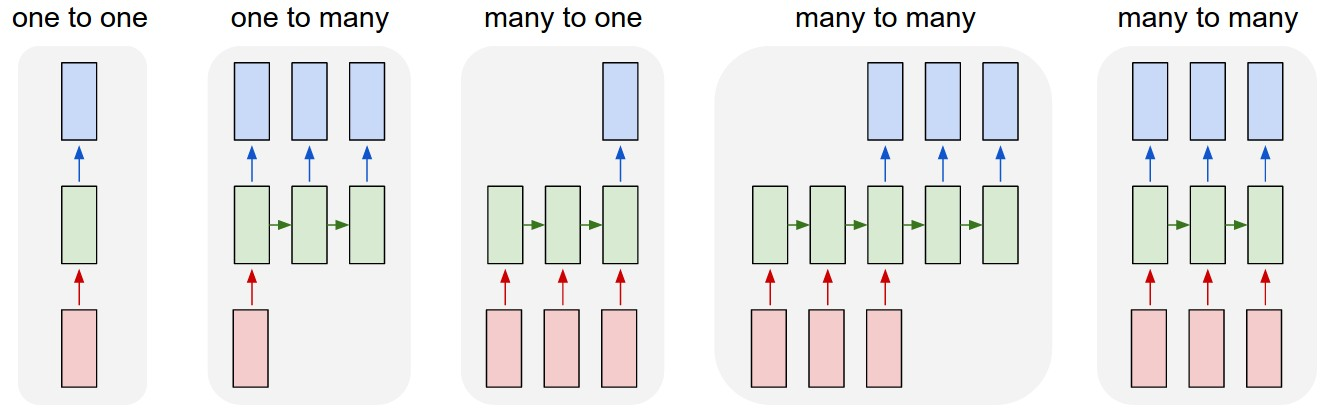
\includegraphics[width=0.6\linewidth,keepaspectratio]{pyt57}
\end{center}

\end{frame}

%%%%%%%%%%%%%%%%%%%%%%%%%%%%%%%%%%%%%%%%%%%%%%%%%%%
\begin{frame}[fragile] \frametitle{Generative networks}

\begin{itemize}
\item One-to-one is a traditional neural network with one input and one output
\item One-to-many is a generative architecture that accepts one input value, and generates a sequence of output values. For example, if we want to train image captioning network that would produce a textual description of a picture, we can a picture as input, pass it through CNN to obtain hidden state, and then have recurrent chain generate caption word-by-word
\item Many-to-one corresponds to RNN architectures we described in the previous unit, such as text classification
\item Many-to-many, or sequence-to-sequence corresponds to tasks such as machine translation, where we have first RNN collect all information from the input sequence into the hidden state, and another RNN chain unrolls this state into the output sequence.
\end{itemize}

\end{frame}

%%%%%%%%%%%%%%%%%%%%%%%%%%%%%%%%%%%%%%%%%%%%%%%%%%%
\begin{frame}[fragile] \frametitle{Character Level Language Modeling}

During training, we need to take some text corpus, and split it into letter sequences.

\begin{lstlisting}
from torchnlp import *
train_dataset,test_dataset,classes,vocab = load_dataset()

def char_tokenizer(words):
    return list(words) #[word for word in words]

counter = collections.Counter()
for (label, line) in train_dataset:
    counter.update(char_tokenizer(line))
vocab = torchtext.vocab.Vocab(counter)

vocab_size = len(vocab)
print(f"Vocabulary size = {vocab_size}")
print(f"Encoding of 'a' is {vocab.stoi['a']}")
print(f"Character with code 13 is {vocab.itos[13]}")

>>>
Vocabulary size = 84
Encoding of 'a' is 4
Character with code 13 is h
\end{lstlisting}

\end{frame}

%%%%%%%%%%%%%%%%%%%%%%%%%%%%%%%%%%%%%%%%%%%%%%%%%%%
\begin{frame}[fragile] \frametitle{Character Level Language Modeling}

Let's see the example of how we can encode the text from our dataset:
\begin{lstlisting}
def enc(x):
    return torch.LongTensor(encode(x,voc=vocab,tokenizer=char_tokenizer))

enc(train_dataset[0][1])

>>>
tensor([43,  4, 11, 11,  2, 26,  5, 23,  2, 38,  3,  4, 10,  9,  2, 31, 11,  4,
        :
         3,  3,  7,  8, 18,  2, 18, 10,  3,  3,  8,  2,  4, 18,  4,  7,  8, 23])
\end{lstlisting}

\end{frame}


%%%%%%%%%%%%%%%%%%%%%%%%%%%%%%%%%%%%%%%%%%%%%%%%%%%
\begin{frame}[fragile] \frametitle{Training a generative RNN}

\begin{itemize}
\item On each step, we will take a sequence of characters of length nchars, and ask the network to generate next output character for each input character:

\begin{center}
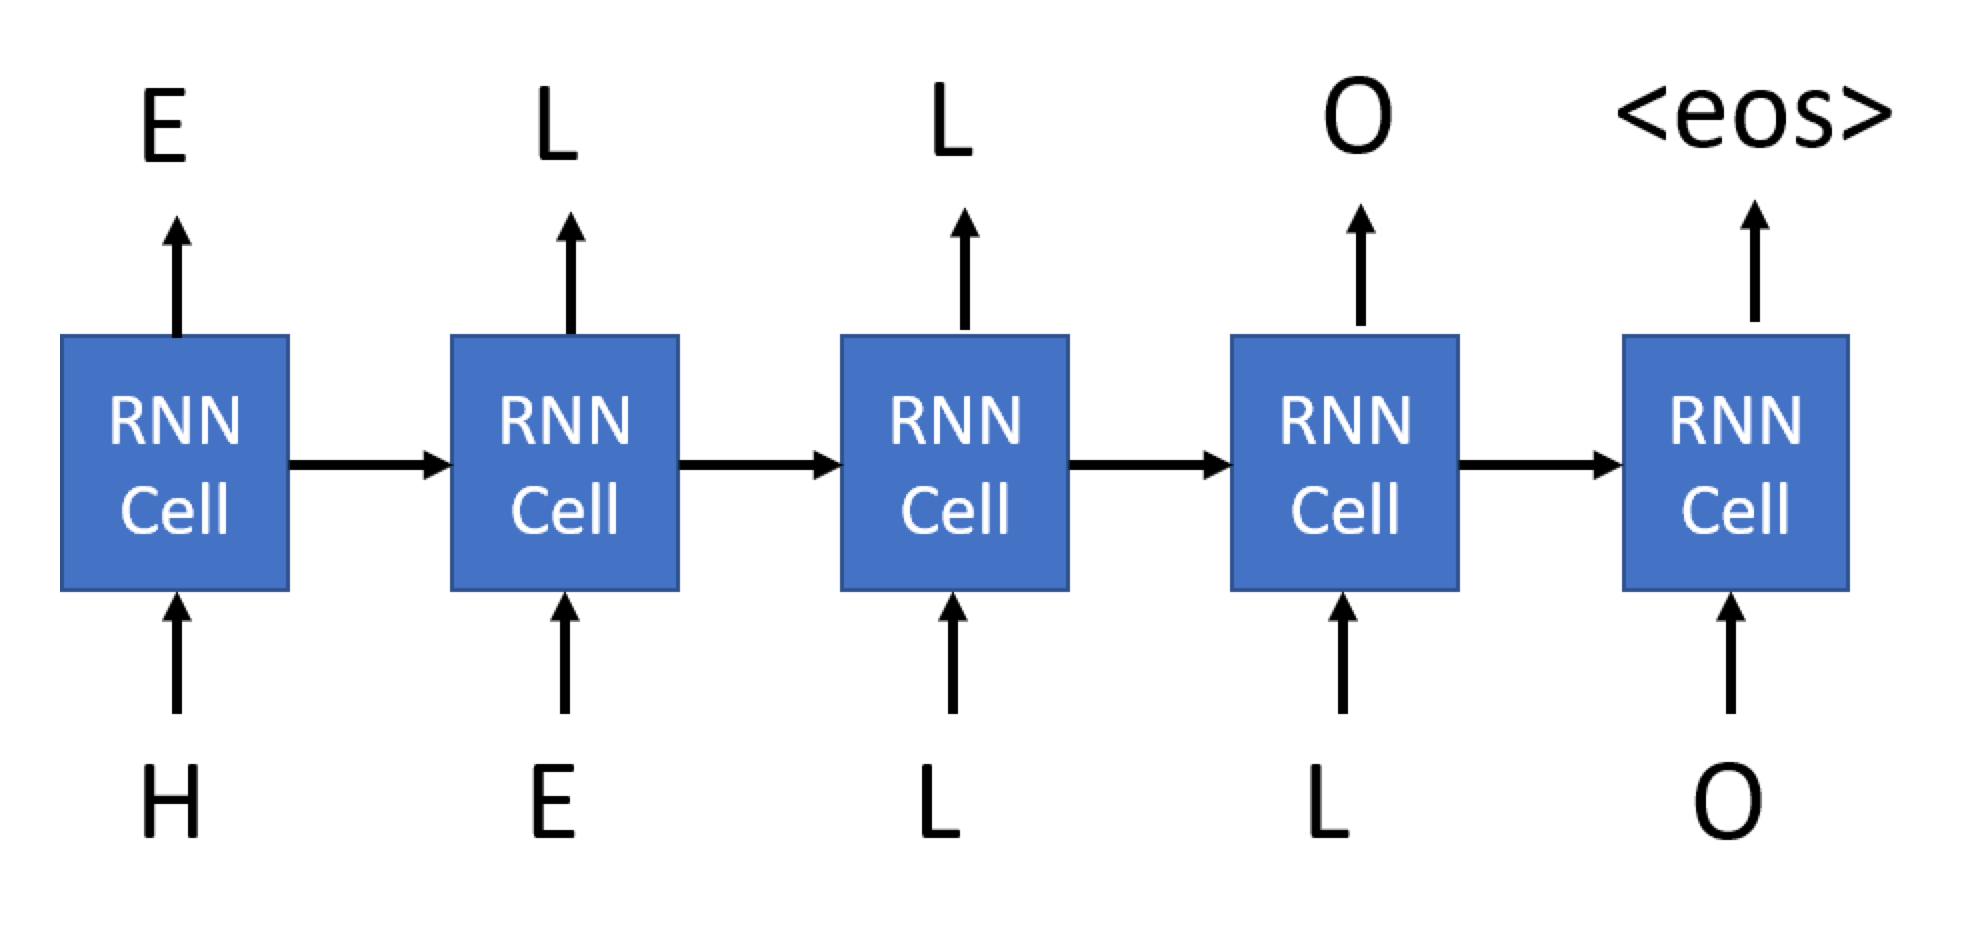
\includegraphics[width=0.6\linewidth,keepaspectratio]{pyt58}
\end{center}

\item Depending on the actual scenario, we may also want to include some special characters, such as end-of-sequence \lstinline|<eos>|. 
\item Each training example will consist of nchars inputs and nchars outputs (which are input sequence shifted one symbol to the left). 
\item Minibatch will consist of several such sequences.
\end{itemize}

\end{frame}

%%%%%%%%%%%%%%%%%%%%%%%%%%%%%%%%%%%%%%%%%%%%%%%%%%%
\begin{frame}[fragile] \frametitle{Mini batches}

\begin{itemize}
\item The way we will generate minibatches is to take each news text of length l, and generate all possible input-output combinations from it (there will be l-nchars such combinations). 
\item They will form one minibatch, and size of minibatches would be different at each training step.
\end{itemize}

\begin{lstlisting}
nchars = 100

def get_batch(s,nchars=nchars):
    ins = torch.zeros(len(s)-nchars,nchars,dtype=torch.long,device=device)
    outs = torch.zeros(len(s)-nchars,nchars,dtype=torch.long,device=device)
    for i in range(len(s)-nchars):
        ins[i] = enc(s[i:i+nchars])
        outs[i] = enc(s[i+1:i+nchars+1])
    return ins,outs

get_batch(train_dataset[0][1])

>>>
(tensor([[43,  4, 11,  ..., 18, 61, 22],...
         [15,  5,  3,  ...,  4,  7,  8]], device='cuda:0'),
 tensor([[ 4, 11, 11,  ..., 61, 22,  4], ...
         [ 5,  3, 10,  ...,  7,  8, 23]], device='cuda:0'))
\end{lstlisting}

\end{frame}

%%%%%%%%%%%%%%%%%%%%%%%%%%%%%%%%%%%%%%%%%%%%%%%%%%%
\begin{frame}[fragile] \frametitle{Generator Network}

\begin{itemize}
\item Because the network takes characters as input, and vocabulary size is pretty small, we do not need embedding layer, one-hot-encoded input can directly go to LSTM cell. 
\item However, because we pass character numbers as input, we need to one-hot-encode them before passing to LSTM. 
\item This is done by calling \lstinline|one_hot| function during forward pass. Output encoder would be a linear layer that will convert hidden state into one-hot-encoded output.
\end{itemize}

\begin{lstlisting}
class LSTMGenerator(torch.nn.Module):
    def __init__(self, vocab_size, hidden_dim):
        super().__init__()
        self.rnn = torch.nn.LSTM(vocab_size,hidden_dim,batch_first=True)
        self.fc = torch.nn.Linear(hidden_dim, vocab_size)

    def forward(self, x, s=None):
        x = torch.nn.functional.one_hot(x,vocab_size).to(torch.float32)
        x,s = self.rnn(x,s)
        return self.fc(x),s
\end{lstlisting}

\end{frame}


%%%%%%%%%%%%%%%%%%%%%%%%%%%%%%%%%%%%%%%%%%%%%%%%%%%
\begin{frame}[fragile] \frametitle{Generator Network}

\begin{itemize}
\item During training, we want to be able to sample generated text. 
\item To do that, we will define generate function that will produce output string of length size, starting from the initial string start.
\end{itemize}

The way it works is the following. 

\begin{itemize}
\item First, we will pass the whole start string through the network, and take output state s and next predicted character out. 
\item Since out is one-hot encoded, we take argmax to get the index of the character nc in the vocabulary, and use itos to figure out the actual character and append it to the resulting list of characters chars. 
\item This process of generating one character is repeated size times to generate required number of characters.
\end{itemize}
\end{frame}

%%%%%%%%%%%%%%%%%%%%%%%%%%%%%%%%%%%%%%%%%%%%%%%%%%%
\begin{frame}[fragile] \frametitle{Generator Network}

\begin{itemize}
\item Now let's do the training! Training loop is almost the same as in all our previous examples, but instead of accuracy we print sampled generated text every 1000 epochs.
\item Special attention needs to be paid to the way we compute loss. 
\item We need to compute loss given one-hot-encoded output out, and expected text \lstinline|text_out|, which is the list of character indices. 
\item Luckily, the \lstinline|cross_entropy| function expects unnormalized network output as first argument, and class number as the second, which is exactly what we have. 
\item It also performs automatic averaging over minibatch size.
\item We also limit the training by \lstinline|samples_to_train samples|, in order not to wait for too long.
\end{itemize}


\begin{lstlisting}
def generate(net,size=100,start='today '):
        chars = list(start)
        out, s = net(enc(chars).view(1,-1).to(device))
        for i in range(size):
            nc = torch.argmax(out[0][-1])
            chars.append(vocab.itos[nc])
            out, s = net(nc.view(1,-1),s)
        return ''.join(chars)
\end{lstlisting}




\end{frame}

%%%%%%%%%%%%%%%%%%%%%%%%%%%%%%%%%%%%%%%%%%%%%%%%%%%
\begin{frame}[fragile] \frametitle{Generator Network}
\begin{lstlisting}
net = LSTMGenerator(vocab_size,64).to(device)

samples_to_train = 10000
optimizer = torch.optim.Adam(net.parameters(),0.01)
loss_fn = torch.nn.CrossEntropyLoss()
net.train()
for i,x in enumerate(train_dataset):
    # x[0] is class label, x[1] is text
    if len(x[1])-nchars<10:
        continue
    samples_to_train-=1
    if not samples_to_train: break
    text_in, text_out = get_batch(x[1])
    optimizer.zero_grad()
    out,s = net(text_in)
    loss = torch.nn.functional.cross_entropy(out.view(-1,vocab_size),text_out.flatten()) #cross_entropy(out,labels)
    loss.backward()
    optimizer.step()
    if i%1000==0:
        print(f"Current loss = {loss.item()}")
        print(generate(net))
\end{lstlisting}

\end{frame}

%%%%%%%%%%%%%%%%%%%%%%%%%%%%%%%%%%%%%%%%%%%%%%%%%%%
\begin{frame}[fragile] \frametitle{Generator Network}

This example already generates some pretty good text but it can be further improved in several ways:

\begin{itemize}
\item Better minibatch generation.
\item Multilayer LSTM.
\item GRU units
\end{itemize}


\begin{lstlisting}
Current loss = 4.442246913909912
today ggrgrgrgrgrgrgrgrgrgrgrgrgrgrgrgrgrgrgrgrgrgrgrgrgrgrgrgrgrgrgrgrgrgrgrgrgrgrgrgrgrgrgrgrgrgrgrgrgrg
Current loss = 2.1178359985351562
today and a could a the to the to the to the to the to the to the to the to the to the to the to the to th
:
Current loss = 1.5444810390472412
today and the counters to the first the counters to the first the counters to the first the counters to th
\end{lstlisting}


\end{frame}

%%%%%%%%%%%%%%%%%%%%%%%%%%%%%%%%%%%%%%%%%%%%%%%%%%%
\begin{frame}[fragile] \frametitle{Attention mechanisms}


\begin{itemize}
\item One major drawback of recurrent networks is that all words in a sequence have the same impact on the result. 
\item This causes sub-optimal performance with standard LSTM encoder-decoder models for sequence to sequence tasks, such as Named Entity Recognition and Machine Translation. 
\item In reality specific words in the input sequence often have more impact on sequential outputs than others.
\item Attention Mechanisms provide a means of weighting the contextual impact of each input vector on each output prediction of the RNN. 
\item The way it is implemented is by creating shortcuts between intermediate states of the input RNN, and output RNN. 
\item In this manner, when generating output symbol $y_t$, we will take into account all input hidden states $h_i$, with different weight coefficients $\alpha_{t,i}$. 

\end{itemize}
\end{frame}

%%%%%%%%%%%%%%%%%%%%%%%%%%%%%%%%%%%%%%%%%%%%%%%%%%%
\begin{frame}[fragile] \frametitle{Attention mechanisms}

\begin{center}
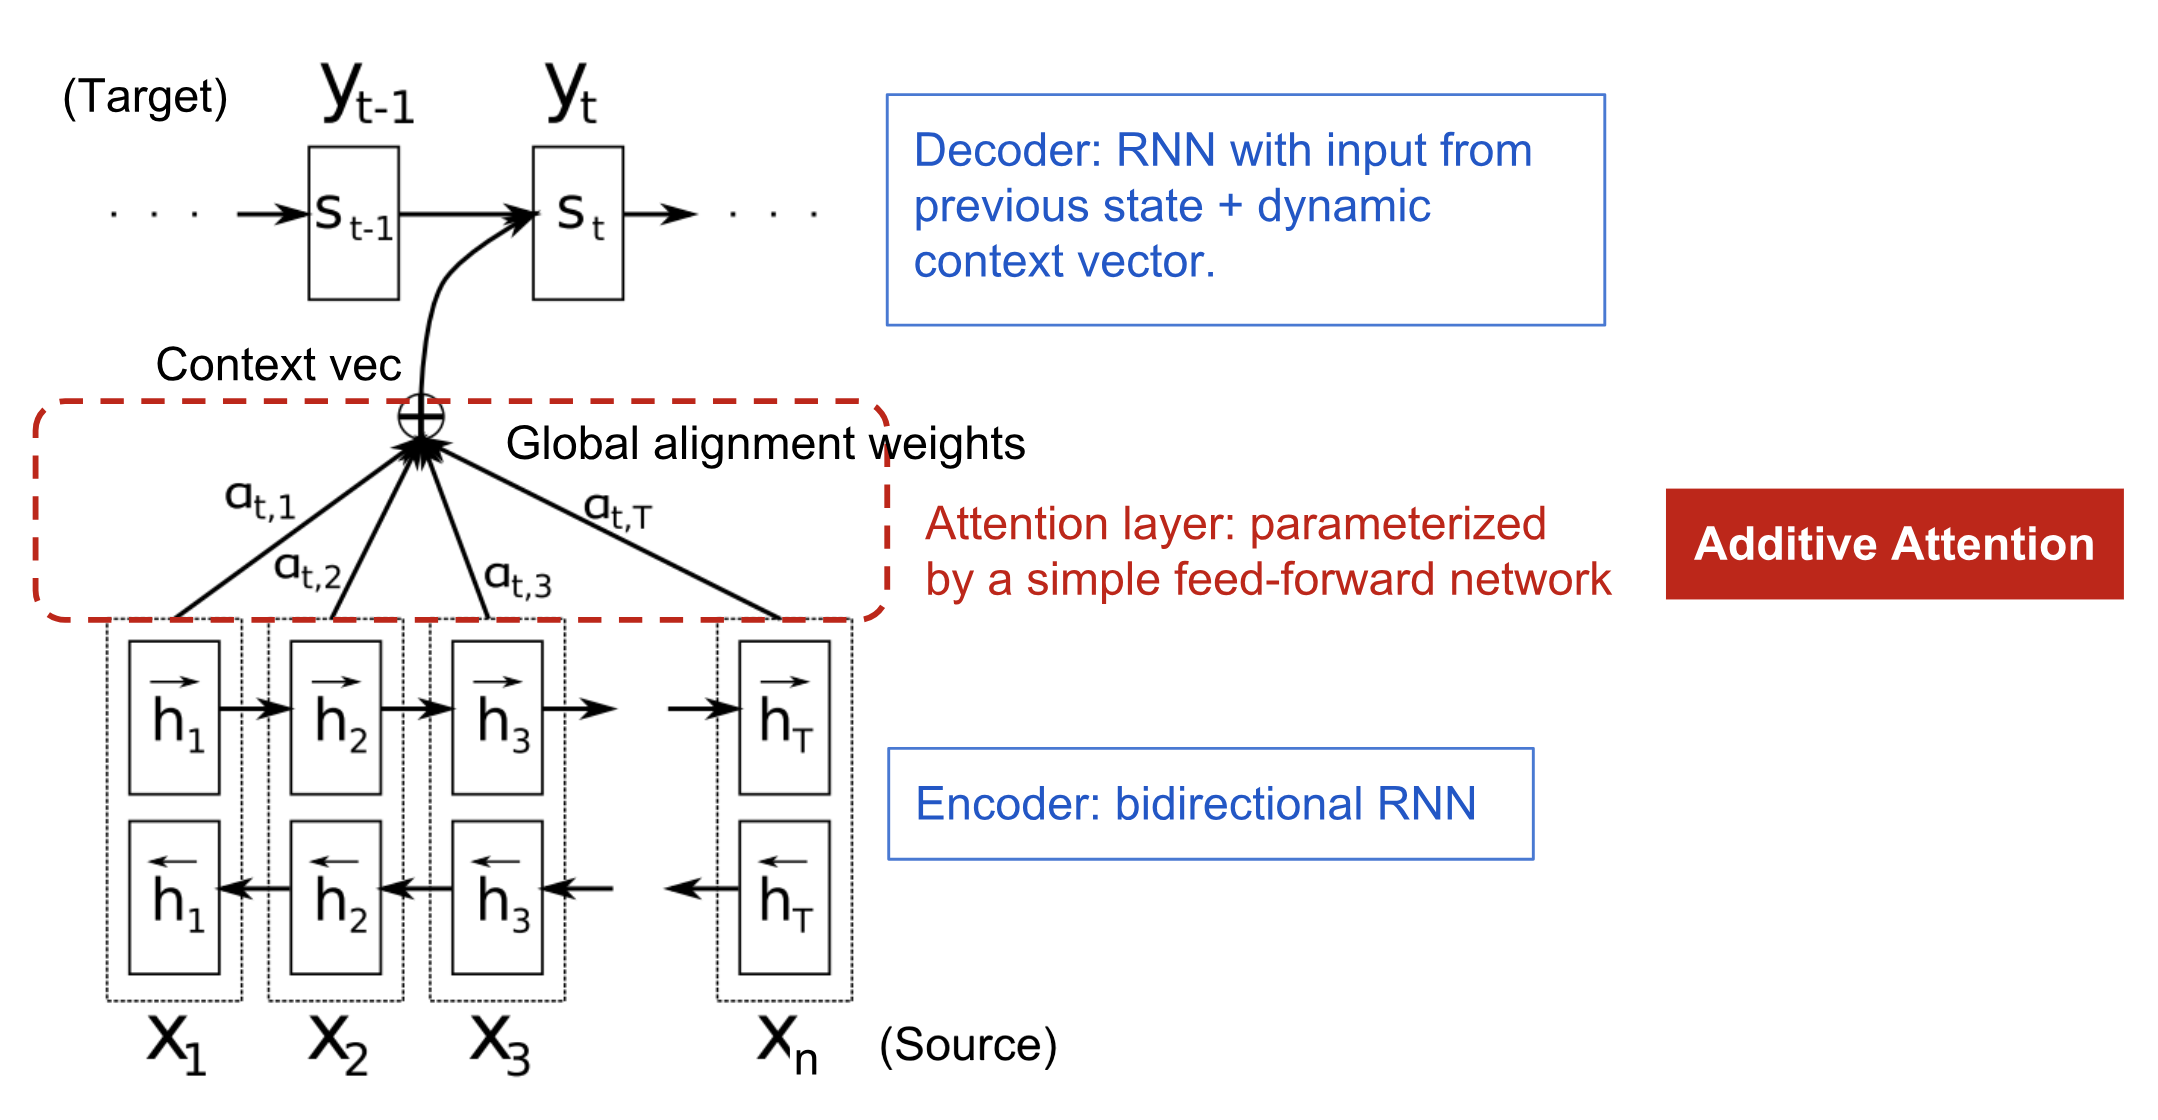
\includegraphics[width=0.9\linewidth,keepaspectratio]{pyt59}
\end{center}

{\tiny The encoder-decoder model with additive attention mechanism in Bahdanau et al., 2015}
\end{frame}

%%%%%%%%%%%%%%%%%%%%%%%%%%%%%%%%%%%%%%%%%%%%%%%%%%%
\begin{frame}[fragile] \frametitle{Attention mechanisms}

Attention matrix $\{\alpha_{i,j}\}$ would represent the degree which certain input words play in generation of a given word in the output sequence. Below is the example of such a matrix:


\begin{center}
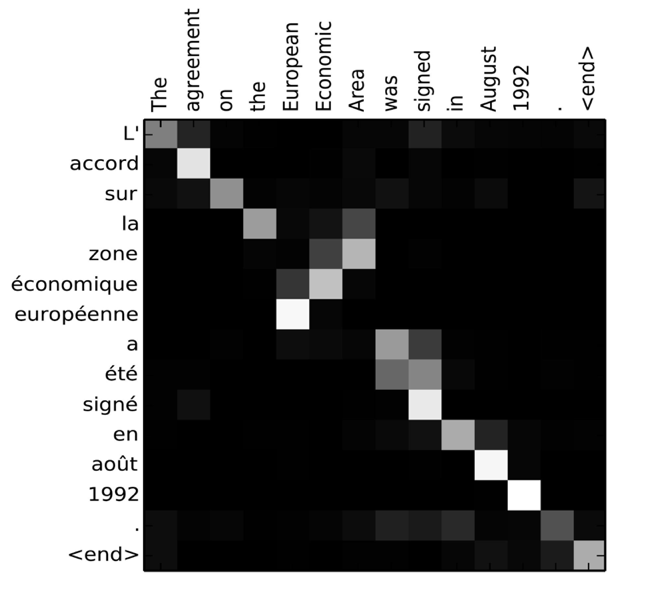
\includegraphics[width=0.5\linewidth,keepaspectratio]{pyt60}
\end{center}

{\tiny The encoder-decoder model with additive attention mechanism in Bahdanau et al., 2015}
\end{frame}

%%%%%%%%%%%%%%%%%%%%%%%%%%%%%%%%%%%%%%%%%%%%%%%%%%%
\begin{frame}[fragile] \frametitle{To Transformers}


\begin{itemize}
\item Adding attention greatly increases the number of model parameters which led to scaling issues with RNNs. 
\item A key constraint of scaling RNNs is that the recurrent nature of the models makes it challenging to batch and parallelize training. 
\item In an RNN each element of a sequence needs to be processed in sequential order which means it cannot be easily parallelized.
\item Adoption of attention mechanisms combined with this constraint led to the creation of the now State of the Art Transformer Models that we know and use today from BERT to OpenGPT3.
\item ATTENTION IS ALL YOU NEED!!
\end{itemize}
\end{frame}

%%%%%%%%%%%%%%%%%%%%%%%%%%%%%%%%%%%%%%%%%%%%%%%%%%%
\begin{frame}[fragile] \frametitle{Transformers}


\begin{itemize}
\item Instead of forwarding the context of each previous prediction into the next evaluation step, transformer models use positional encodings and attention to capture the context of a given input with in a provided window of text.
\item Since each input position is mapped independently to each output position, transformers can parallelize better than RNNs, which enables much larger and more expressive language models. 
\item Each attention head can be used to learn different relationships between words that improves downstream Natural Language Processing tasks.
\end{itemize}

\begin{center}
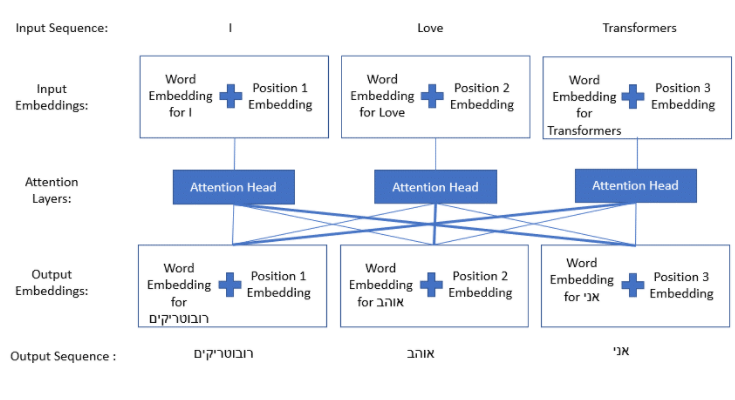
\includegraphics[width=0.5\linewidth,keepaspectratio]{pyt61}
\end{center}
\end{frame}

%%%%%%%%%%%%%%%%%%%%%%%%%%%%%%%%%%%%%%%%%%%%%%%%%%%
\begin{frame}[fragile] \frametitle{BERT}

Bidirectional Encoder Representations from Transformers

\begin{itemize}
\item is a very large multi layer transformer network with 12 layers for BERT-base, and 24 for BERT-large. The model is first pre-trained on large corpus of text data (WikiPedia + books) using unsupervised training (predicting masked words in a sentence). 
\item During pre-training the model absorbs significant level of language understanding which can then be leveraged with other datasets using fine tuning, called transfer learning.
\end{itemize}

\end{frame}

%%%%%%%%%%%%%%%%%%%%%%%%%%%%%%%%%%%%%%%%%%%%%%%%%%%
\begin{frame}[fragile] \frametitle{BERT}

\begin{center}
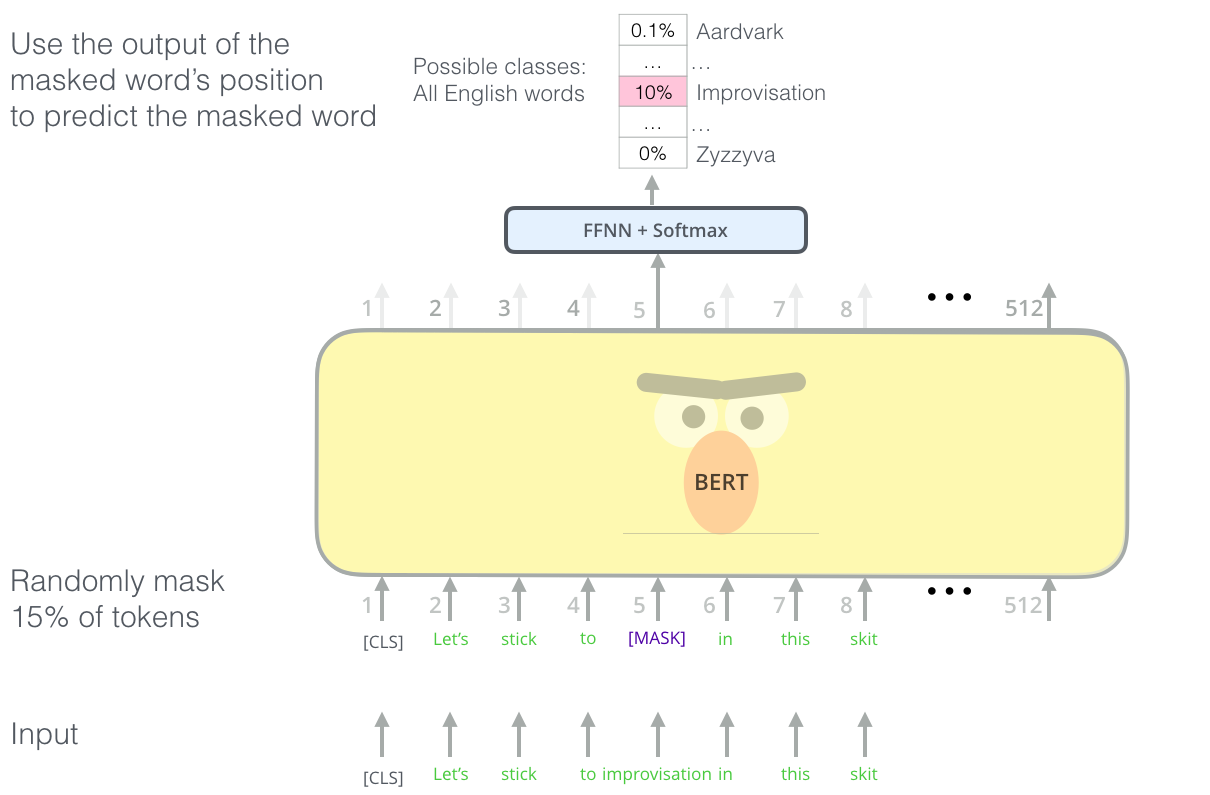
\includegraphics[width=0.5\linewidth,keepaspectratio]{pyt62}
\end{center}

There are many variations of Transformer architectures including BERT, DistilBERT. BigBird, OpenGPT3 and more that can be fine tuned. The HuggingFace package provides repository for training many of these architectures with PyTorch.
\end{frame}
